% Options for packages loaded elsewhere
\PassOptionsToPackage{unicode}{hyperref}
\PassOptionsToPackage{hyphens}{url}
%
\documentclass[
]{article}
\usepackage{lmodern}
\usepackage{amssymb,amsmath}
\usepackage{ifxetex,ifluatex}\usepackage[
  lambda,
  advantage,
  operators,
  sets,
  adversary,
  probability,
  notions,
  primitives,
  oracles,
  keys
]{cryptocode}

\usepackage{float}
\usepackage[margin=1in]{geometry}
\usepackage{amsmath,amssymb}
\usepackage{tikz}
\usetikzlibrary{arrows.meta,positioning,calc}

\ifnum 0\ifxetex 1\fi\ifluatex 1\fi=0 % if pdftex
  \usepackage[T1]{fontenc}
  \usepackage[utf8]{inputenc}
  \usepackage{textcomp} % provide euro and other symbols
\else % if luatex or xetex
  \usepackage{unicode-math}
  \defaultfontfeatures{Scale=MatchLowercase}
  \defaultfontfeatures[\rmfamily]{Ligatures=TeX,Scale=1}
\fi
% Use upquote if available, for straight quotes in verbatim environments
\IfFileExists{upquote.sty}{\usepackage{upquote}}{}
\IfFileExists{microtype.sty}{% use microtype if available
  \usepackage[]{microtype}
  \UseMicrotypeSet[protrusion]{basicmath} % disable protrusion for tt fonts
}{}
\makeatletter
\@ifundefined{KOMAClassName}{% if non-KOMA class
  \IfFileExists{parskip.sty}{%
    \usepackage{parskip}
  }{% else
    \setlength{\parindent}{0pt}
    \setlength{\parskip}{6pt plus 2pt minus 1pt}}
}{% if KOMA class
  \KOMAoptions{parskip=half}}
\makeatother
\usepackage{xcolor}
\IfFileExists{xurl.sty}{\usepackage{xurl}}{} % add URL line breaks if available
\IfFileExists{bookmark.sty}{\usepackage{bookmark}}{\usepackage{hyperref}}
\hypersetup{
  hidelinks,
  pdfcreator={LaTeX via pandoc}}
\urlstyle{same} % disable monospaced font for URLs
\setlength{\emergencystretch}{3em} % prevent overfull lines
\providecommand{\tightlist}{%
  \setlength{\itemsep}{0pt}\setlength{\parskip}{0pt}}
\setcounter{secnumdepth}{-\maxdimen} % remove section numbering
\usepackage[
  lambda,
  advantage,
  operators,
  sets,
  adversary,
  probability,
  notions,
  primitives,
  oracles,
  keys
]{cryptocode}

\author{}
\date{}

\begin{document}

\hypertarget{pkeet}{%
\section{PKEET}\label{pkeet}}

\begin{quote}
Nhan\_laptop
\end{quote}

\hypertarget{motivation}{%
\subsection{Motivation}\label{motivation}}

In this blog, I'll introduce a PKEET (Public Key Encryption with
Equality Test) scheme that allows two parties to encrypt their data and
later test if the encrypted data is equal without revealing the actual
data. This is particularly useful in scenarios where privacy is a
concern, such as in secure voting systems or confidential data sharing.

\hypertarget{definition}{%
\subsection{Definition}\label{definition}}

\hypertarget{hibe-scheme}{%
\subsubsection{HIBE Scheme}\label{hibe-scheme}}

Full HIBE, Which I introduced in the \href{../IBE-HIBE/IBE-HIBE.md}{HIBE
blog}. In this blog, we define a HIBE scheme as:

\begin{itemize}
\item
  \(Setup(1^\lambda) \rightarrow (mpk, msk)\): mpk contains the public
  parameters and msk contains the master secret key.
\item
  \(KeyExt({sk}_{id},ID') \rightarrow {sk}_{ID'}\)
\item
  \(Enc(mpk,ID,M) \rightarrow ct\)
\item
  \(Dec({sk}_{ID}, ct) \rightarrow M'\)
\end{itemize}

\hypertarget{digital-signature-scheme}{%
\subsubsection{Digital Signature
Scheme}\label{digital-signature-scheme}}

There are three PPT algorithms in a digital signature scheme: 1.
\textbf{Key Generation (KeyGen) \(G(\lambda)\)}:

\[G(\lambda) \rightarrow ({vk}_s, {sk}_s)\]

\begin{itemize}
\tightlist
\item
  \({vk}_s\): verification key
\item
  \({sk}_s\): signing key
\end{itemize}

\begin{enumerate}
\def\labelenumi{\arabic{enumi}.}
\setcounter{enumi}{1}
\tightlist
\item
  Signing (Sign) \(S({sk}_s, m)\):
\end{enumerate}

\[S({sk}_s, m) \rightarrow \sigma\]

\begin{enumerate}
\def\labelenumi{\arabic{enumi}.}
\setcounter{enumi}{2}
\tightlist
\item
  Verification (Verify) \(V({vk}_s, m, \sigma)\):
\end{enumerate}

\[V({vk}_s, m, \sigma) \rightarrow \{0, 1\}\]

\hypertarget{strong-unforgeability}{%
\subsubsection{Strong Unforgeability}\label{strong-unforgeability}}

A signature scheme \(Sig = (G, S, V)\) is strongly unforgeable under an
adaptive chosen message attack if for any PPT adversary A, the
probability that the adversary wins in the following game with the
challenger C is negligible in the security parameter λ:

\begin{enumerate}
\def\labelenumi{\arabic{enumi}.}
\item
  \textbf{Setup}: \(C\) run \(G(\lambda)\) to generate
  \(({vk}_s, {sk}_s)\) and sends \({vk}_s\) to A.
\item
  \(Signature Queries\):

  \begin{itemize}
  \tightlist
  \item
    A can query the signing oracle \(S({sk}_s, \cdot)\) on any message
    \(m_i\) of its choice and receives the signature \(\sigma_i\).
  \item
    Note:

    \begin{itemize}
    \tightlist
    \item
      A can query the same message multiple times and receive different
      signatures.
    \item
      A can query the signing oracle on a message \(m_i\) that it has
      already queried before.
    \end{itemize}
  \end{itemize}
\item
  \textbf{Output}: A outputs a message-signature pair
  \((m^*, \sigma^*)\).
\end{enumerate}

The adversary A wins if: - \(V({vk}_s, m^*, \sigma^*) = 1\) -
\((m^*, \sigma^*)\) is not equal to any of the message-signature pairs
\((m_i, \sigma_i)\) that A queried to the signing oracle.

\hypertarget{public-key-encryption-with-equality-test-pkeet}{%
\subsubsection{Public Key Encryption with Equality Test
(PKEET)}\label{public-key-encryption-with-equality-test-pkeet}}

There are six PPT algorithms in a PKEET scheme
(\(PKEET = (Setup, KeyGen, Enc, Dec, Td,Test)\)):

\begin{enumerate}
\def\labelenumi{\arabic{enumi}.}
\tightlist
\item
  \textbf{Setup}: \(Setup(1^\lambda) \rightarrow pp,\ M\)

  \begin{itemize}
  \tightlist
  \item
    Generates public parameters \(pp\) based on the security parameter
    \(\lambda\).
  \item
    \(M\): message space
  \end{itemize}
\item
  \textbf{Key Generation}: \(KeyGen(pp) \rightarrow (pk, sk)\)

  \begin{itemize}
  \tightlist
  \item
    Generates a public key \(pk\) and a secret key \(sk\).
  \item
    \((pk_i)\): public key of user \((U_i)\)
  \item
    \((sk_i)\): secret key of user \((U_i)\)
  \item
    \((td_i)\): trapdoor generated from \((sk_i)\) by \((Td(sk_i))\)
  \end{itemize}
\item
  \textbf{Encryption}: \(Enc(pk, m) \rightarrow c\)

  \begin{itemize}
  \tightlist
  \item
    Encrypts a message \(m \in M\) using the public key \(pk\) to
    produce a ciphertext \(c\).
  \end{itemize}
\item
  \textbf{Decryption}: \(Dec(sk, c) \rightarrow m\)

  \begin{itemize}
  \tightlist
  \item
    Decrypts a ciphertext \(c\) using the secret key \(sk\) to produce
    the original message \(m\).
  \end{itemize}
\item
  \textbf{Trapdoor Generation}: \(Td(sk) \rightarrow td\)

  \begin{itemize}
  \tightlist
  \item
    Generates a trapdoor \(td\) using the secret key \(sk\).
  \end{itemize}
\item
  \textbf{Equality Test}:
  \(Test(td_i, ct_i, td_j, ct_j) \rightarrow \{0, 1\}\)

  \begin{itemize}
  \tightlist
  \item
    Tests whether two ciphertexts \(c_1\) and \(c_2\) encrypt the same
    message using the trapdoor \(td\).
  \item
    Returns 1 if they are equal, and 0 otherwise.
  \end{itemize}
\end{enumerate}

Correctness:

\begin{enumerate}
\def\labelenumi{\arabic{enumi}.}
\item
  \(Pr[Test({td}_i,{ct_i},{td}_j,{ct_j}) \rightarrow 1] = 1\) if
  \(m_i = m_j\) and \(i = j\) or \(i \neq j\)
\item
  \$Pr{[}Test(\{td\}\_i,\{ct\_i\},\{td\}\_j,\{ct\_j\}) \rightarrow 1{]}
  = 1 \$ negligible.
\end{enumerate}

\hypertarget{security-model}{%
\subsection{Security Model}\label{security-model}}

There are two types defined:

\begin{enumerate}
\def\labelenumi{\arabic{enumi}.}
\tightlist
\item
  \textbf{Type-I Adversary}:

  \begin{itemize}
  \tightlist
  \item
    The adversary can obtain the trapdoor for the target user's
    ciphertext and so can test equality with the challenge ciphertext.
  \item
    The aim of this type is trying to reveal the plaintext of the
    challenge ciphertext.
  \end{itemize}
\item
  \textbf{Type-II Adversary}:

  \begin{itemize}
  \tightlist
  \item
    In contrast, the aim of this type is trying to distinguish the
    challenge ciphertext which message between two candidates.
  \end{itemize}
\end{enumerate}

\hypertarget{ow-cca2-against-type-i-adversaries}{%
\subsubsection{OW-CCA2 against Type-I
Adversaries}\label{ow-cca2-against-type-i-adversaries}}

\begin{enumerate}
\def\labelenumi{\arabic{enumi}.}
\item
  \textbf{Setup}: \(C\) runs \(Setup(1^\lambda)\rightarrow params\),
  sends \(params\) to \(A\). Then \(C\) runs
  \(KeyGen(params) \rightarrow (pk, sk)\) and sends \(pk\) to \(A\).
\item
  \textbf{Phase 1}:
\end{enumerate}

\begin{itemize}
\tightlist
\item
  \(O^{sk}\): input index \(i\) and output \(U_i\)'s secret key
  \(sk_i\).
\item
  \(O^{Dec}\): input pair \((i, c)\) and output \(Dec(sk_i, c)\).
\item
  \(O^{Td}\): input index \(i\) and output \(U_i\)'s trapdoor \(td_i\)
  by running \(Td(sk_i)\rightarrow td_i\) with \(sk_i\).
\end{itemize}

Constraints: \(A\) cannot query \(O^{sk}\) for target index.

\begin{enumerate}
\def\labelenumi{\arabic{enumi}.}
\setcounter{enumi}{2}
\item
  \textbf{Challenge}: \(C\) chooses a random message \(M\) from the
  message space \(M\), \(Enc(pk_{t}, M) \rightarrow c_{t}^*\) and sends
  \(c_{t}^*\) to \(A\).
\item
  \textbf{Phase 2}: Same as Phase 1, the constraints:
\end{enumerate}

\begin{itemize}
\tightlist
\item
  \(A\) cannot query \(O^{sk}\) for target index.
\item
  the pair of the index t and the ciphertext \(c_{t}^*\) cannot be
  queried to \(O^{Dec}\) .
\end{itemize}

\begin{enumerate}
\def\labelenumi{\arabic{enumi}.}
\setcounter{enumi}{4}
\tightlist
\item
  \textbf{Output}: \(A\) outputs a message \(M'\) and wins if
  \(M' = M\).
\end{enumerate}

The advantage of \(A\) is defined as:
\[Adv_{A}^{OW-CCA2}(\lambda) = |Pr[M' = M] - \frac{1}{|M|}|\]

\hypertarget{ind-cca2-against-type-ii-adversaries}{%
\subsubsection{IND-CCA2 against Type-II
Adversaries}\label{ind-cca2-against-type-ii-adversaries}}

\begin{enumerate}
\def\labelenumi{\arabic{enumi}.}
\item
  \textbf{Setup}: \(C\) runs \(Setup(1^\lambda)\rightarrow params\),
  sends \(params\) to \(A\). Then \(C\) runs
  \(KeyGen(params) \rightarrow (pk, sk)\) and sends \(pk\) to \(A\).
\item
  \textbf{Phase 1}: the same as Phase 1 in OW-CCA2 against Type-I
  Adversaries, except the constraints: cannot query \(O^{Td}\) for
  target index.
\item
  \textbf{Challenge}: \(A\) chooses two messages \(M_0, M_1\) from the
  message space \(M\), \(C\) chooses a random bit \(b \in \{0, 1\}\),
  then \(Enc(pk_{t}, M_b) \rightarrow c_{t}^*\) and sends \(c_{t}^*\) to
  \(A\).
\item
  \textbf{Phase 2}: Same as Phase 1, the constraints:
\end{enumerate}

\begin{itemize}
\tightlist
\item
  the index t cannot be queried to \(O^{Td}\) and the key extraction
  oracle \(O^{sk}\).
\item
  the pair of the index t and the ciphertext \(c_{t}^*\) cannot be
  queried to \(O^{Dec}\).
\end{itemize}

\begin{enumerate}
\def\labelenumi{\arabic{enumi}.}
\setcounter{enumi}{4}
\tightlist
\item
  \textbf{Guess}: \(A\) outputs a bit \(b'\) and wins if \(b' = b\).
\end{enumerate}

The advantage of \(A\) is defined as:
\[Adv_{A}^{IND-CCA2}(\lambda) = |Pr[b' = b] - \frac{1}{2}|\]

\hypertarget{pkeet-construction}{%
\subsection{PKEET Construction}\label{pkeet-construction}}

2-level HIBE scheme: - \([{ID}_1. {ID}_2]\) denotes an identity in the
2-level HIBE scheme, where \({ID}_1\) is the identity of the first level
and \({ID}_2\) is the identity of the second level.

\begin{verbatim}
root
├── [0]
│    └── [0.vks]  -> encrypt M
└── [1]
     └── [1.vks]  -> encrypt H(M)
\end{verbatim}

\begin{itemize}
\tightlist
\item
  \(HIBE=(Setup, KeyExtract,Enc, Dec)\).
\end{itemize}

Applied CHK transformation to IBE-IND-sID-CPA scheme to get
PKEET-IND-CCA2 scheme.

CHK transformation scheme:

\begin{enumerate}
\def\labelenumi{\arabic{enumi}.}
\item
  Generate a signature key pair \(({vk}_s, {sk}_s)\)
\item
  Encrypt the message \(m\) using the IBE scheme with the verification
  key \({vk}_s\) as the identity.
\item
  Sign the resulting ciphertext using the signing key \({sk}_s\) to
  produce a signature \(\sigma\).
\end{enumerate}

The proposed encryption scheme (combine 2-level HIBE and signature
scheme \(Sig =(G,S,V)\)) is defined as follows:

\begin{enumerate}
\def\labelenumi{\arabic{enumi}.}
\item
  \(G(\lambda)\rightarrow ({vk}_s, {sk}_s)\).
\item
  \(Enc(mpk, [0.{vk}_s],M)\rightarrow c_0\).
\item
  \(Enc(mpk, [1.{vk}_s],H(M))\rightarrow c_1\).
\item
  \(S({sk}_s, c_0||c_1)\rightarrow \sigma\).
\item
  \(ct = ({vk}_s, c_0, c_1, \sigma)\)
\end{enumerate}

\hypertarget{full-pkeet-construction}{%
\subsubsection{Full PKEET Construction}\label{full-pkeet-construction}}

\begin{itemize}
\tightlist
\item
  \(Setup(\lambda)\): generates:
\end{itemize}

\begin{enumerate}
\def\labelenumi{\arabic{enumi}.}
\item
  a 2-level HIBE scheme \(HIBE=(Setup, KeyExt,Enc, Dec)\)
\item
  a hash function \(H: \{0, 1\}^* \rightarrow M\)
\item
  a digital signature scheme \(Sig = (G, S, V)\)
\end{enumerate}

\begin{itemize}
\item
  \(KeyGen(params)\): on input params it runs
  \(Setup(\lambda)\rightarrow (mpk,msk)\) and output a public key
  \(pk = mpk\) and a secret key \(sk = msk\).
\item
  \(Enc(pk,M):\) input pk and M:
\end{itemize}

\begin{enumerate}
\def\labelenumi{\arabic{enumi}.}
\tightlist
\item
  \(G(\lambda)\rightarrow ({vk}_s, {sk}_s)\)
\item
  \(Enc(mpk, [0.{vk}_s],M)\rightarrow c_0\)
\item
  \(Enc(mpk, [1.{vk}_s],H(M))\rightarrow c_1\)
\item
  \(S({sk}_s, c_0||c_1)\rightarrow \sigma\)
\end{enumerate}

it outputs \(ct = ({vk}_s, c_0, c_1, \sigma)\)

\begin{itemize}
\tightlist
\item
  \(Dec(sk, ct)\): input sk and ct:
\end{itemize}

\begin{enumerate}
\def\labelenumi{\arabic{enumi}.}
\item
  Run \(KeyExt(sk,[i,{vk}_s])\rightarrow {sk}_i\) for \(i \in \{0, 1\}\)
\item
  Decrypt \(c_0,c_1\) by running \(Dec({sk}_0, c_0)\rightarrow M'\) and
  \(Dec({sk}_1, c_1)\rightarrow h'\)
\item
  Check if \(H(M') = h'\), and
  \(V({vk}_s, c_0||c_1, \sigma)\rightarrow 1\), then output \(M'\),
  otherwise output \(\perp\).
\end{enumerate}

\begin{itemize}
\item
  \(Td(sk):\) input \({sk}_i\): runs
  \(KeyExt({sk}_i,1)\rightarrow {sk}_{i,1}\), and outputs
  \(td = {sk}_{i,1}\).
\item
  \(Test({td}_i, ct_i, {td}_j, ct_j)\): input
  \(td_i, ct_i, td_j, ct_j\):
\end{itemize}

\begin{enumerate}
\def\labelenumi{\arabic{enumi}.}
\item
  parse \({ct}_k\) to \(({vk}_{s,k}, c_{k,0}, c_{k,1}, \sigma_k)\) for
  \(k \in \{i, j\}\)
\item
  run \(KeyExt({td}_k,[1.{vk}_{s,k}])\rightarrow {sk}_{k,1}\) for
  \(k \in \{i, j\}\)
\item
  run \(Dec({sk}_{k,[1.{vk}_{s,k}]}, c_{k,1})\rightarrow h_k'\) for
  \(k \in \{i, j\}\)
\end{enumerate}

if \(h_i' = h_j'\) then output 1, otherwise output 0.

correctness: - Theorem 1: if HIBE scheme, scheme \(Sig\) are correct,
and the employed hash function \(H\) is collision-resistant, then the
proposed PKEET scheme is correct.

\hypertarget{security-analysis}{%
\subsection{Security Analysis}\label{security-analysis}}

\hypertarget{theorem-2}{%
\subsubsection{Theorem 2:}\label{theorem-2}}

if: - HIBE scheme is IND-sID-CPA secure 2-level HIBE scheme, - \(Sig\)
is strongly unforgeable one-time signature scheme, then: the proposed
PKEET scheme is IND-CCA2 secure against Type-II adversaries.

The advantage of any Type-II adversary \(A\) against the proposed PKEET
scheme is bounded:

\[
2\cdot \epsilon_{HIBE}+ \frac{3\cdot \epsilon_{Sig}}{2} 
\]

which: - \(\epsilon_{HIBE}\): there is no PPT adversary that can break
the IND-sID-CPA security of the 2-level HIBE scheme with at least
advantage \(\epsilon_{HIBE}\). - \(\epsilon_{Sig}\): there is no PPT
adversary that can break the strong unforgeability of the one-time
signature scheme with at least advantage \(\epsilon_{Sig}\).

\hypertarget{security-game}{%
\paragraph{Security game:}\label{security-game}}

\begin{itemize}
\tightlist
\item
  setup: let \(N\) be the number of users in the system, t be the index
  of the target user,
  \(ct*_t = (vk_{s,t}*,C_{t,0}*,C_{t,1}*,\sigma_t*)\) be the challenge
  ciphertext fot the user \(U_t\).
\end{itemize}

\textbf{Game 0}: the original game for the type-II adversary.

\textbf{Game 1}: The same as Game 0, except that if \(A\) queries the
oracle \(O^{dec}(t,\cdot)\) on
\(ct_t=(vk_{s,t},C_{t,0},C_{t,1},\sigma_t)\) such that
\(vk_{s,t} = vk_{s,t}*\), \(ct_t \neq ct*_t\), and
\(V(vk_{s,t},|C_{t,0}||C_{t,1}||\sigma_t)\rightarrow 1\), then
challenger \(C\) stops an interaction and sets \(A's\) answer at random.

\textbf{Game 2}: The same as Game 1, except for the challenger's respone
in the challenge phase. The origin challenge ciphertext \(ct_t*\) has
the form \((vk_{s,t}*, C_{t,0}*, C_{t,1}*, \sigma_t*)\), where
\(G(\lambda)\rightarrow ({vk}_{s,t}*, {sk}_{s,t}*)\),
\(Enc(pk_t, [0,{vk}_{s,t}*],M_b)\rightarrow C_{t,0}*\) and
\(Enc(pk_t, [1,{vk}_{s,t}*],H(M_b))\rightarrow C_{t,1}*\),
\(S({sk}_{s,t}*, c_{t,0}*||c_{t,1}*)\rightarrow \sigma_t*\), which b is
a random bit chosen by C.

C tosses a two unbiased coins a,b. -
\(a= 0 \rightarrow M_b, \ H(M_{1-b})\) -
\(a= 1 \rightarrow M_{1-b}, \ H(M_b)\)

The advantage of A in \(Game_i\) be \(\epsilon_i\) for
\(i \in \{0,1,2\}\), that is \(\epsilon_i = |\Pr[G_i]-\frac{1}{2}|\).

We prove the theorem by sequence of lemmas.

\textbf{lemma 1}:
\(\epsilon_0 - \epsilon_1 \leq \frac{3\cdot \epsilon_{Sig}}{2}\)

The event \(E_1\) that \(A\) queries the oracle \(O^{dec}(t,\cdot)\) on
\(ct_t=(vk_{s,t},C_{t,0},C_{t,1},\sigma_t)\) such that
\(vk_{s,t} = vk_{s,t}*\), \(ct_t \neq ct*_t\), and
\(V(vk_{s,t},|C_{t,0}||C_{t,1}||\sigma_t)\rightarrow 1\), then \(C\)
should stops an interaction and sets \(A's\) answer at random.

So:

\[
\begin{equation}
\begin{aligned}
\epsilon_1
&= \left|\Pr[\mathcal{G}_1]-\frac{1}{2}\right| \\[2mm]
&= \left|
    \Pr[\mathcal{G}_1\mid E_1]\Pr[E_1]
    +
    \Pr[\mathcal{G}_1\mid \neg E_1]\Pr[\neg E_1]
    -
    \frac{1}{2}
   \right| \\[2mm]
&= \left|
    \frac{1}{2}\Pr[E_1]
    +
    \Pr[\mathcal{G}_0\wedge \neg E_1]
    -
    \frac{1}{2}
   \right| \\[2mm]
&= \left|
    \frac{1}{2}\Pr[E_1]
    +
    \Pr[\mathcal{G}_0]
    -
    \Pr[\mathcal{G}_0\wedge E_1]
    -
    \frac{1}{2}
   \right| \\[2mm]
&= \left|
    \left(\Pr[\mathcal{G}_0]-\frac{1}{2}\right)
    +
    \left(\frac{1}{2}\Pr[E_1]
    -
    \Pr[\mathcal{G}_0\wedge E_1]\right)
   \right| \\[2mm]
&\ge
   \left|\Pr[\mathcal{G}_0]-\frac{1}{2}\right|
   -
   \left|
    \frac{1}{2}\Pr[E_1]
    -
    \Pr[\mathcal{G}_0\wedge E_1]
   \right| \\[2mm]
&\ge
   \epsilon_0
   -
   \frac{3}{2}\Pr[E_1].
\end{aligned}
\end{equation}
\]

Note:

\[
\Pr[\mathcal{G}_1]
=
\Pr[\mathcal{G}_1\mid E_1]\Pr[E_1]
+
\Pr[\mathcal{G}_1\mid \neg E_1]\Pr[\neg E_1].
\]

The third line uses the definition of Game 1. If the bad event \((E_1)\)
occurs, the game aborts or returns a random bit. Therefore, the
adversary wins with probability:

\[
\Pr[\mathcal{G}_1\mid E_1]=\frac{1}{2}.
\]

If \((E_1)\) does not occur, then Game 1 and Game 0 are identical from
the adversary's view. Hence:

\[
\Pr[\mathcal{G}_1\wedge \neg E_1]
=
\Pr[\mathcal{G}_0\wedge \neg E_1].
\]

The fourth line uses the decomposition:

\[
\Pr[\mathcal{G}_0\wedge \neg E_1]
=
\Pr[\mathcal{G}_0]
-
\Pr[\mathcal{G}_0\wedge E_1].
\]

The fifth line only groups the expression into two parts:

\[
\left(\Pr[\mathcal{G}_0]-\frac{1}{2}\right)
\]

and

\[
\left(\frac{1}{2}\Pr[E_1]-\Pr[\mathcal{G}_0\wedge E_1]\right).
\]

The sixth line uses the reverse triangle inequality:

\[
|X+Y|\ge |X|-|Y|.
\]

Finally, since:

\[
\mathcal{G}_0\wedge E_1 \subseteq E_1,
\]

we have:

\[
\Pr[\mathcal{G}_0\wedge E_1]\le \Pr[E_1].
\]

Therefore:

\[
\begin{aligned}
\left|
\frac{1}{2}\Pr[E_1]
-
\Pr[\mathcal{G}_0\wedge E_1]
\right|
&\le
\frac{1}{2}\Pr[E_1]
+
\Pr[\mathcal{G}_0\wedge E_1] \\[1mm]
&\le
\frac{1}{2}\Pr[E_1]+\Pr[E_1] \\[1mm]
&=
\frac{3}{2}\Pr[E_1].
\end{aligned}
\]

Since:

\[
\epsilon_0
=
\left|\Pr[\mathcal{G}_0]-\frac{1}{2}\right|,
\]

we obtain:

\[
\boxed{
\epsilon_1
\ge
\epsilon_0
-
\frac{3}{2}\Pr[E_1].
}
\]

This means that the adversary's advantage in Game 1 is almost the same
as in Game 0, except for the probability of the bad event \((E_1)\).
Therefore, if \((\Pr[E_1])\) is negligible, then the transition from
Game 0 to Game 1 only loses a negligible amount of advantage.

\textbf{Proof}:

\[
Pr[E_1] \le \epsilon_{Sig}
\]

\begin{figure}[ht]
\centering

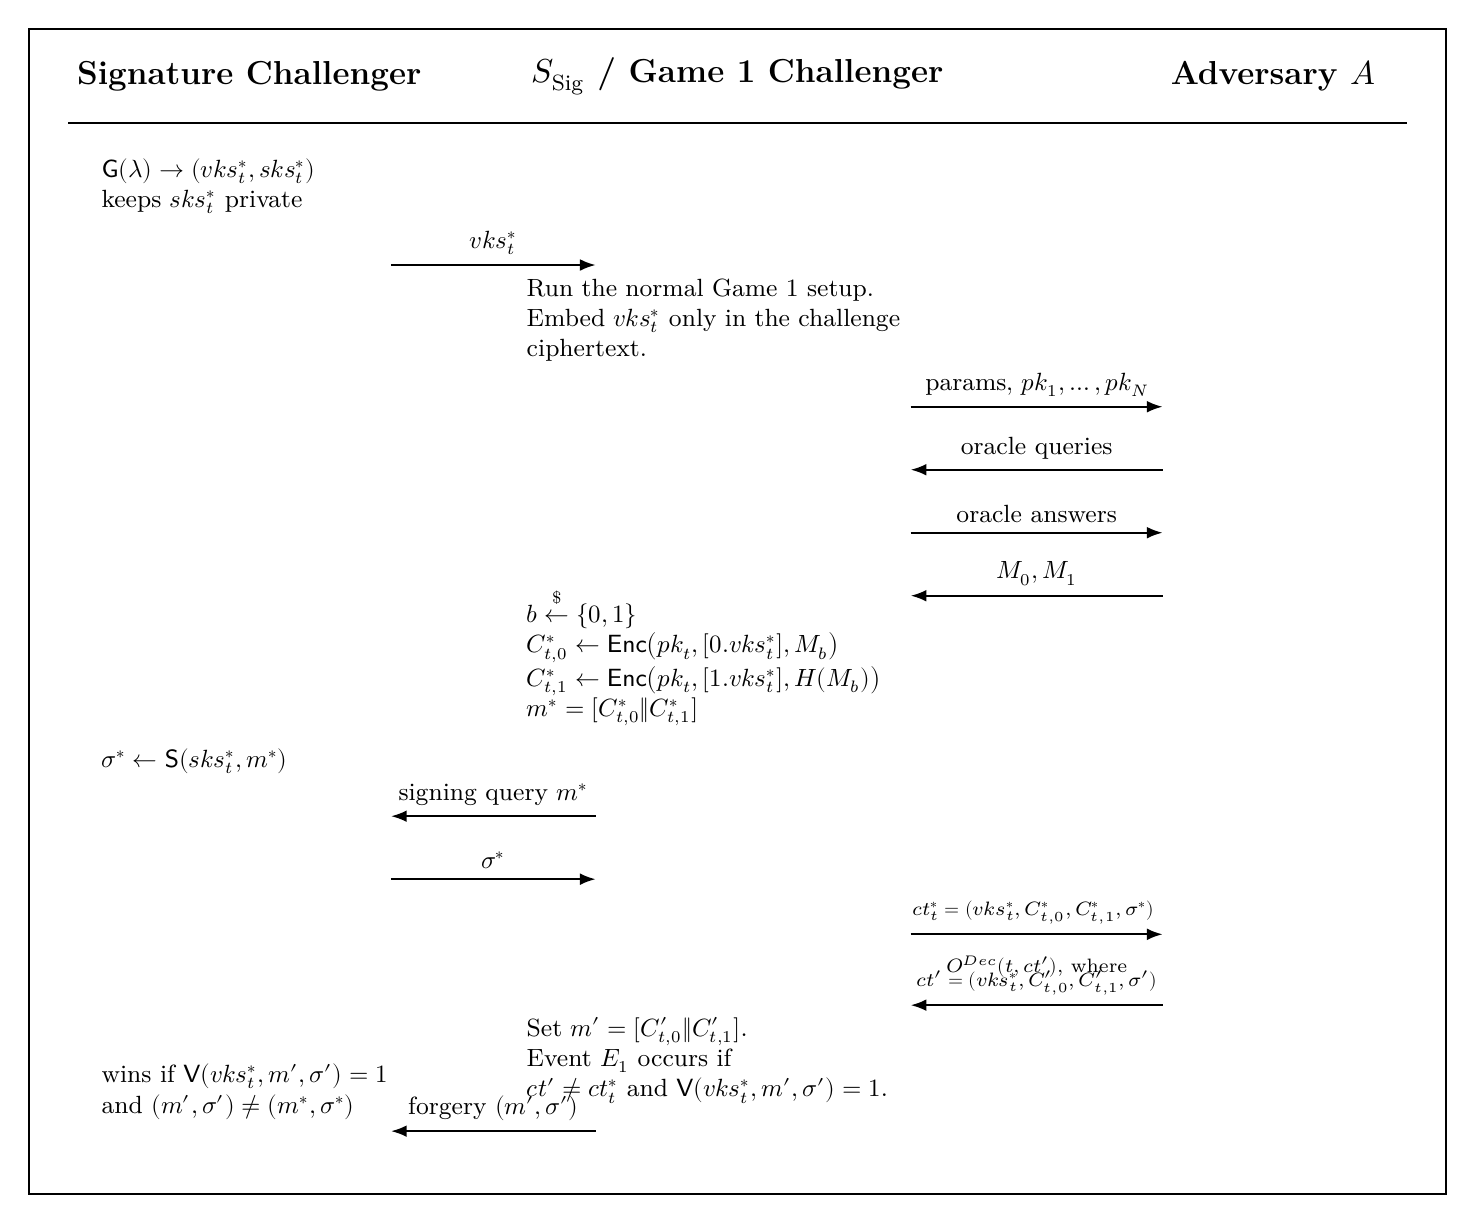
\begin{tikzpicture}[
    >=Latex,
    font=\small,
    hdr/.style={font=\bfseries\large},
    note/.style={align=left},
    simnote/.style={align=left, text width=5.3cm},
    arr/.style={-{Latex[length=2mm]}, thick},
    revarr/.style={{Latex[length=2mm]}-, thick}
]

% =====================================================
% Stakeholder columns
% =====================================================

\def\xSig{2.8}
\def\xSim{9.0}
\def\xAdv{15.8}

% Arrow zones
\def\xSSL{4.6}
\def\xSSR{7.2}

\def\xSAL{11.2}
\def\xSAR{14.4}

% =====================================================
% Outer box
% =====================================================

\draw[thick] (0,0) rectangle (18,-14.8);
\draw[thick] (0.5,-1.2) -- (17.5,-1.2);

% =====================================================
% Headers
% =====================================================

\node[hdr] at (\xSig,-0.6)
{Signature Challenger};

\node[hdr] at (\xSim,-0.6)
{$S_{\mathrm{Sig}}$ / Game 1 Challenger};

\node[hdr] at (\xAdv,-0.6)
{Adversary $A$};

% =====================================================
% Strong-unforgeability setup
% =====================================================

\node[note, anchor=west] at (0.8,-2.0)
{
$\mathsf{G}(\lambda)
 \rightarrow
 (vks_t^*,sks_t^*)$\\
keeps $sks_t^*$ private
};

\draw[arr]
    (\xSSL,-3.0)
    --
    node[above] {$vks_t^*$}
    (\xSSR,-3.0);

% =====================================================
% PKEET Game 1 setup
% =====================================================

\node[simnote, anchor=west] at (6.2,-3.7)
{
Run the normal Game 1 setup.\\
Embed $vks_t^*$ only in the challenge ciphertext.
};

\draw[arr]
    (\xSAL,-4.8)
    --
    node[above]
    {$\mathrm{params},\,pk_1,\ldots,pk_N$}
    (\xSAR,-4.8);

\draw[revarr]
    (\xSAL,-5.6)
    --
    node[above] {oracle queries}
    (\xSAR,-5.6);

\draw[arr]
    (\xSAL,-6.4)
    --
    node[above] {oracle answers}
    (\xSAR,-6.4);

% =====================================================
% Challenge messages
% =====================================================

\draw[revarr]
    (\xSAL,-7.2)
    --
    node[above] {$M_0,M_1$}
    (\xSAR,-7.2);

% =====================================================
% Challenge ciphertext generation
% =====================================================

\node[simnote, anchor=west] at (6.2,-8.0)
{
$b \overset{\$}{\leftarrow}\{0,1\}$

$C_{t,0}^{*}
 \gets
 \mathsf{Enc}
 \bigl(pk_t,[0.vks_t^*],M_b\bigr)$

$C_{t,1}^{*}
 \gets
 \mathsf{Enc}
 \bigl(pk_t,[1.vks_t^*],H(M_b)\bigr)$

$m^*
 =
 [C_{t,0}^{*}\Vert C_{t,1}^{*}]$
};

% =====================================================
% One signing query
% =====================================================

\draw[revarr]
    (\xSSL,-10.0)
    --
    node[above] {signing query $m^*$}
    (\xSSR,-10.0);

\node[note, anchor=west] at (0.8,-9.3)
{
$\sigma^*
 \gets
 \mathsf{S}(sks_t^*,m^*)$
};

\draw[arr]
    (\xSSL,-10.8)
    --
    node[above] {$\sigma^*$}
    (\xSSR,-10.8);

% =====================================================
% PKEET challenge ciphertext
% =====================================================

\draw[arr]
    (\xSAL,-11.5)
    --
    node[
        midway,
        above,
        align=center,
        font=\scriptsize
    ]
    {
    $ct_t^*
     =
     (vks_t^*,
      C_{t,0}^*,
      C_{t,1}^*,
      \sigma^*)$
    }
    (\xSAR,-11.5);

% =====================================================
% Event E1: malicious decryption query
% =====================================================

\draw[revarr]
    (\xSAL,-12.4)
    --
    node[
        midway,
        above,
        align=center,
        font=\scriptsize
    ]
    {
    $O^{Dec}(t,ct')$, where\\[-1mm]
    $ct'=(vks_t^*,C'_{t,0},C'_{t,1},\sigma')$
    }
    (\xSAR,-12.4);

\node[simnote, anchor=west] at (6.2,-13.1)
{
Set
$m'=[C'_{t,0}\Vert C'_{t,1}]$.

Event $E_1$ occurs if

$ct'\neq ct_t^*$ and
$\mathsf{V}(vks_t^*,m',\sigma')=1$.
};

% =====================================================
% Forgery output
% =====================================================

\draw[revarr]
    (\xSSL,-14.0)
    --
    node[above]
    {forgery $(m',\sigma')$}
    (\xSSR,-14.0);

\node[note, anchor=west] at (0.8,-13.5)
{
wins if
$\mathsf{V}(vks_t^*,m',\sigma')=1$\\
and
$(m',\sigma')\neq(m^*,\sigma^*)$
};

\end{tikzpicture}

\caption{
Reduction used to prove
$\Pr[E_1]<\varepsilon_{\mathrm{Sig}}$.
The simulator embeds the verification key from the
strong-unforgeability game into the PKEET challenge ciphertext
and uses an $E_1$ decryption query as a signature forgery.
}
\label{fig:E1-reduction}

\end{figure}


\begin{itemize}
\tightlist
\item
  S\_Sig receives \(vks*\) from signature challenger.
\item
  S\_Sig runs Game 1 for A.
\item
  In the challenge ciphertext, set \(vks_t* = vks*\).
\item
  S\_Sig creates \(C_t,0*\) and \(C_t,1*\) normally.
\item
  S\_Sig asks its signing oracle to sign \(m*=[C_t,0*||C_t,1*]\).
\item
  S\_Sig gives \(ct_t*\) to A.
\item
  If A causes E1, extract \((m', sigma')\) and output it as a forgery.
\end{itemize}

Hence \(Pr[E_1]\) should be less than \(\epsilon_{Sig}\) by the
assumption that there is no PPT adversary that breaks the strong
unforgeability of the signature scheme with at least \(\epsilon_{Sig}\)
probability.

so:

\[
\epsilon_0 - \epsilon_1 \leq \frac{3\cdot \epsilon_{Sig}}{2}
\]

\textbf{lemma 2}:
\(\epsilon_1 - \epsilon_2 \leq 2\cdot \epsilon_{HIBE}\)

Game:

% \begin{verbatim}
% C_HIBE                         S_HIBE                              A
%    |                              |                                |
%    |                              |-- generate (sks_t^*,vks_t^*)  |
%    |                              |-- choose alpha in {0,1}       |
%    |<-- target ID [alpha.vks_t^*]-|                                |
%    |                              |                                |
%    |-- mpk ---------------------->|                                |
%    |                              |-- set pk_t = mpk              |
%    |                              |-- generate keys for i != t    |
%    |                              |-- params, all public keys --->|
%    |                              |                                |
%    |                              |<------ oracle queries --------|
%    |                              |------ answers ---------------->|
%    |                              |                                |
%    |                              |<------ challenge M0,M1 -------|
%    |                              |                                |
%    |   HIBE challenge happens     |                                |
%    |                              |-- build PKEET challenge ------>|
%    |                              |                                |
%    |                              |<------ output b' -------------|
%    |<-- output b' ----------------|                                |
% \end{verbatim}
\begin{figure}[ht]
\centering
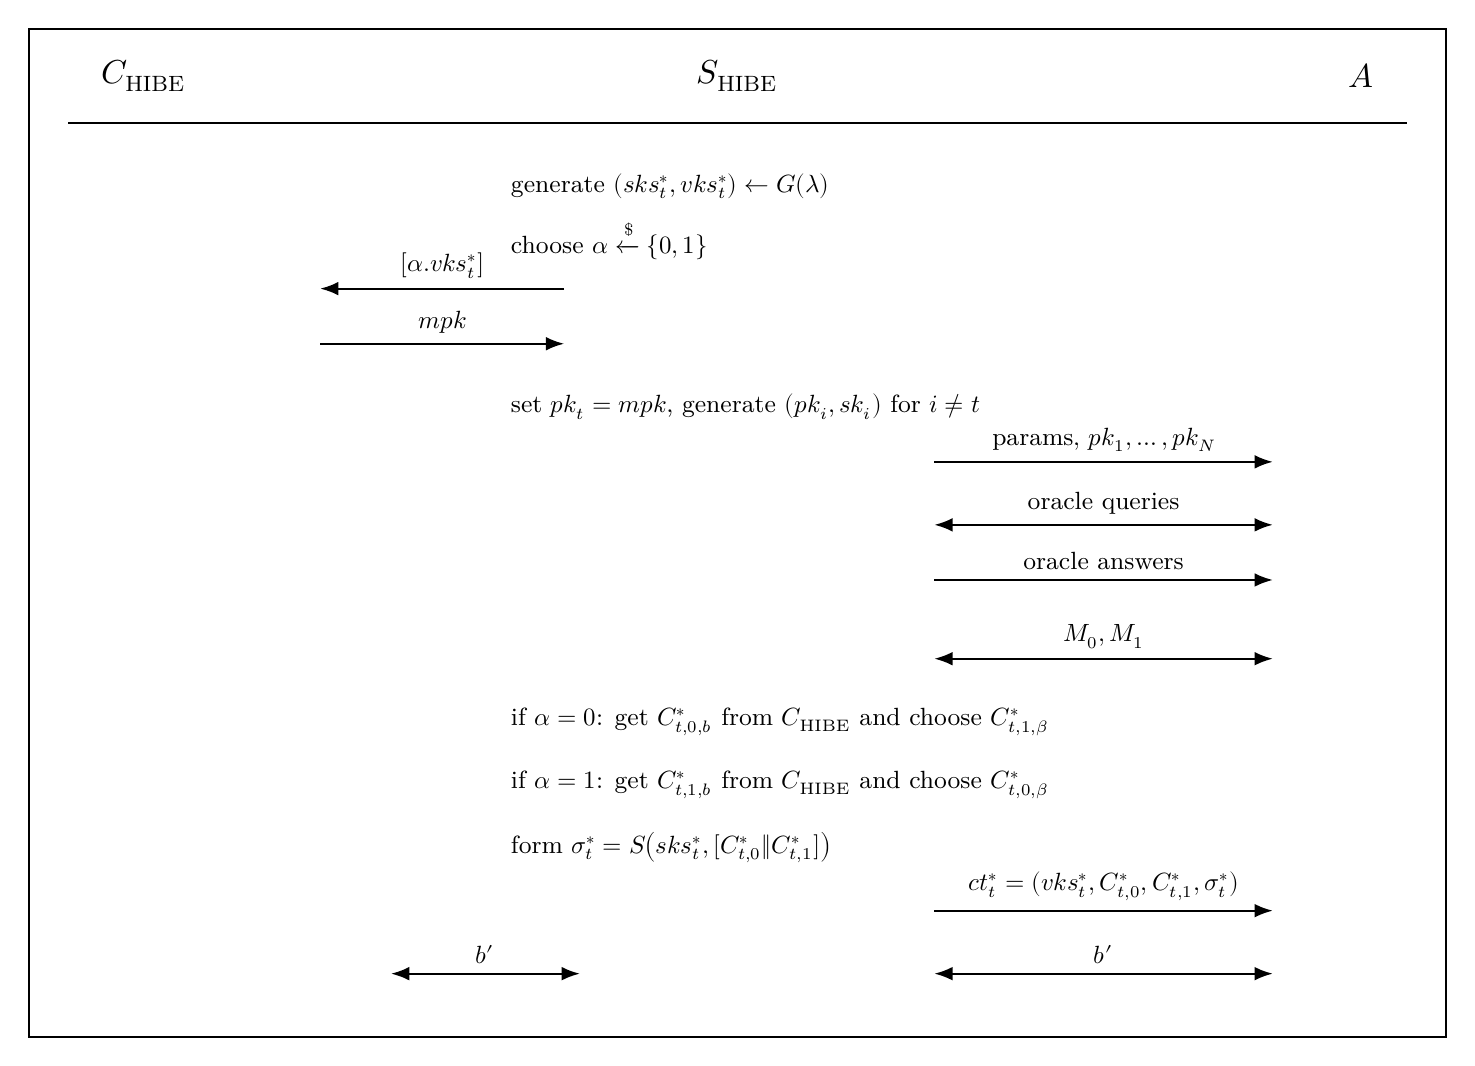
\begin{tikzpicture}[
    >=Latex,
    font=\small,
    hdr/.style={font=\bfseries\large},
    note/.style={align=left},
    arr/.style={-Latex, thick},
    rev/.style={<-Latex, thick}
]
\def\xChal{1.5}
\def\xSim{9.0}
\def\xAdv{16.5}
% Khung được kéo xuống từ -11 thành -12.8
\draw[thick] (0,0) rectangle (18,-12.8);
\draw[thick] (0.5,-1.2) -- (17.5,-1.2);

% =====================================================
% Stakeholders
% =====================================================

\node[hdr, anchor=west] at (0.8,-0.6)
    {$C_{\mathrm{HIBE}}$};

\node[hdr] at (9,-0.6)
    {$S_{\mathrm{HIBE}}$};

\node[hdr, anchor=east] at (17.2,-0.6)
    {$A$};

% =====================================================
% Initialization
% =====================================================

\node[note, anchor=west] at (6.0,-2.0)
    {generate $(sks_t^{*},vks_t^{*}) \gets G(\lambda)$};

\node[note, anchor=west] at (6.0,-2.7)
    {choose $\alpha \xleftarrow{\$}\{0,1\}$};

% S_HIBE -> C_HIBE
% S_HIBE -> C_HIBE
\draw[arr]
    (\xSim-2.2,-3.3)
    --
    node[above] {$[\alpha.vks_t^{*}]$}
    (\xChal+2.2,-3.3);

% C_HIBE -> S_HIBE
% C_HIBE -> S_HIBE
\draw[arr]
    (\xChal+2.2,-4.0)
    --
    node[above] {$mpk$}
    (\xSim-2.2,-4.0);

% =====================================================
% Setup
% =====================================================

\node[note, anchor=west] at (6.0,-4.8)
{
    set $pk_t=mpk$, generate $(pk_i,sk_i)$ for $i\neq t$
};

\draw[arr]
    (11.5,-5.5)
    --
    node[above] {$\mathrm{params},\,pk_1,\ldots,pk_N$}
    (15.8,-5.5);

% =====================================================
% Oracle phase
% =====================================================

\draw[rev]
    (11.5,-6.3)
    --
    node[above] {oracle queries}
    (15.8,-6.3);

\draw[arr]
    (11.5,-7.0)
    --
    node[above] {oracle answers}
    (15.8,-7.0);

% =====================================================
% Challenge phase
% =====================================================

\draw[rev]
    (11.5,-8.0)
    --
    node[above] {$M_0,M_1$}
    (15.8,-8.0);

\node[note, anchor=west] at (6.0,-8.8)
{
    if $\alpha=0$:
    get $C_{t,0,b}^{*}$ from $C_{\mathrm{HIBE}}$
    and choose $C_{t,1,\beta}^{*}$
};

\node[note, anchor=west] at (6.0,-9.6)
{
    if $\alpha=1$:
    get $C_{t,1,b}^{*}$ from $C_{\mathrm{HIBE}}$
    and choose $C_{t,0,\beta}^{*}$
};

\node[note, anchor=west] at (6.0,-10.4)
{
    form
    $\sigma_t^{*}
      =
      S\!\left(
        sks_t^{*},
        [C_{t,0}^{*}\Vert C_{t,1}^{*}]
      \right)$
};

% =====================================================
% PKEET challenge
% =====================================================

\draw[arr]
    (11.5,-11.2)
    --
    node[above]
    {
        $ct_t^{*}
        =
        (vks_t^{*},
         C_{t,0}^{*},
         C_{t,1}^{*},
         \sigma_t^{*})$
    }
    (15.8,-11.2);

% A -> S_HIBE
\draw[rev]
    (11.5,-12.0)
    --
    node[above] {$b'$}
    (15.8,-12.0);

% S_HIBE -> C_HIBE
\draw[rev]
    (4.6,-12.0)
    --
    node[above] {$b'$}
    (7.0,-12.0);

\end{tikzpicture}

\caption{Simulator $S_{\mathrm{HIBE}}$ in the proof of Lemma~2.}
\label{fig:lemma2-simulator}
\end{figure}


We construct a simulator \(S_{HIBE}\) that breaks the IND-sID-CPA
security HIBE by Using A.

Denote the challenger of the IND-sID-CPA security game for HIBE as
\(C_{HIBE}\).

\begin{itemize}
\tightlist
\item
  \textbf{Setup}:
\end{itemize}

\begin{enumerate}
\def\labelenumi{\arabic{enumi}.}
\tightlist
\item
  \(S_{HIBE}\): generates a signature key pair \((vks_t^*, sks_t^*)\)
  and chooses a random bit \(\alpha \in \{0, 1\}\).
\item
  \(S_{HIBE}\) sends the target identity \([{\alpha}, vks_t^*]\) to
  \(C_{HIBE}\).
\item
  \(C_{HIBE}\) generates the master public key \(mpk\) and sends it to
  \(S_{HIBE}\)
\item
  \(S_{HIBE}\) sets \(pk_t = mpk\) and run
  \(Setup(\lambda)\rightarrow (pk_i, sk_i)\) for all \(i \neq t\) and
  sends the parameters, all \(pk_i\) to \(S_{HIBE}\).
\end{enumerate}

\begin{itemize}
\item
  \textbf{Phase 1}: \(S_{HIBE}\) answers all oracle queries from A by
  using the oracles of \(C_{HIBE}\) and the secret keys for all
  \(i \neq t\). If A issues a decryption query on a valid ciphertext
  using \(vk_{s,t}*\), then \(S_{HIBE}\) stops the interaction and
  outputs a random bit.
\item
  \textbf{challenge}: A sends two messages \(M_0, M_1\) to \(S_{HIBE}\).
\end{itemize}

\begin{enumerate}
\def\labelenumi{\arabic{enumi}.}
\tightlist
\item
  if a = 0, then \(S_{HIBE}\) sends \(M_0,M_1\) to \(C_{HIBE}\) to get
  the challenge ciphertext \(C_{t,0,b}^*\) which \(b\) chosen by
  \(C_{HIBE}\), and selects a random bit \[\beta \in \{0, 1\}\]. Send to
  \(A\):
\end{enumerate}

\[
ct_t^* = (vk_{s,t}^*, C_{t,0,b}^*, C_{t,1,\beta}^*= Enc(pk_t,[1\cdot vk_{s,t}^*],H(M_\beta)), \sigma_t^*)
\]

\begin{enumerate}
\def\labelenumi{\arabic{enumi}.}
\setcounter{enumi}{1}
\tightlist
\item
  if a = 1, send \(H(M_1), H(M_0)\), \(C_{t,1,b}^*\)\ldots{}
\end{enumerate}

\begin{itemize}
\tightlist
\item
  \textbf{Guess}: As for the challenge ciphertext, if \(b'=\beta\), the
  challenge ciphertext has the same form as that of Game 1 . Otherwise,
  the challenge ciphertext has the same form as that of Game 2. Hence
  the advantage of \(S_{HIBE}\) can be computed as follows:
\end{itemize}

\[
\begin{equation}
\begin{aligned}
\epsilon_{HIBE} &\ge Adv_{S_{HIBE}\cdot HIBE}^{IND-sID-CPA}(\lambda)\\
&= \left|\Pr[b' = b] - \frac{1}{2}\right|\\
&= \left|\frac{1}{2}\cdot(Pr[b'=b\mod b=\beta] + Pr[b'=b\mod b\neq \beta]) - \frac{1}{2}\right|\\
&= \frac{1}{2}\cdot\left|PR(\mathcal{G}_1)+ Pr(\mathcal{G}_2) - 1\right|\\
&= \frac{1}{2}\cdot\left|(Pr(\mathcal{G}_1)-\frac{1}{2}) + (Pr(\mathcal{G}_2)-\frac{1}{2})\right|\\
&\ge \frac{1}{2}\cdot\left|(Pr(\mathcal{G}_1)-\frac{1}{2})\right| - \frac{1}{2}\cdot\left|(Pr(\mathcal{G}_2)-\frac{1}{2})\right|\\
&= \frac{1}{2}\cdot\epsilon_1 - \frac{1}{2}\cdot\epsilon_2
\end{aligned}
\end{equation}
\]

\textbf{lemma 3}: \(\epsilon_2 = 0\)

In the challenge phase, C computes the challenge ciphertext differently
according to the choice of a. If a=0 uses \(M_b\) and \(H(M_{1-b})\), if
a=1 uses \(M_{1-b}\) and \(H(M_b)\). Even A khown the messages, A cannot
distinguish, since a is completely hidden from viewpoint of A. Hence
\(e_2 = 0\).

Overall, we have:

\[
\epsilon_0 \leq 2\cdot \epsilon_{HIBE}+ \frac{3\cdot \epsilon_{Sig}}{2}
\]

\hypertarget{theorem-3}{%
\subsubsection{Theorem 3:}\label{theorem-3}}

If HIBE is an IND-sID-CPA secure 2-level HIBE scheme, H is a one-way
hash function, and Sig is a strongly unforgeable one-time signature
scheme, then the proposed PKEET scheme is OW-CCA2 secure against Type-I
adversaries in the standard model.

If there is no PPT adversary that can break the IND-sID-CPA security of
the 2-level HIBE scheme with at least advantage \(\epsilon_{HIBE}\),
there is no PPT adversary that can break the strong unforgeability of
the one-time signature scheme with at least advantage
\(\epsilon_{Sig}\), and there is no PPT adversary that can break the
one-wayness of the hash function with at least advantage \(\epsilon_H\),
then the advantage of any Type-I adversary \(A\) against the proposed
PKEET scheme is bounded:

\[
4\cdot \epsilon_{HIBE}+ \epsilon_H + \epsilon_{Sig}
\]

Similarly, we can prove the theorem by sequence of lemmas, and games are
defined as follows:

\textbf{Game 0}: the original OW-CCA2 game .

\textbf{Game 1}: the same as Game 0, except that if \(A\) queries the
oracle \(O^{dec}(t,\cdot)\) on
\(ct_t=(vk_{s,t},C_{t,0},C_{t,1},\sigma_t)\) such that
\(vk_{s,t} = vk_{s,t}*\), \(ct_t \neq ct*_t\), and
\(V(vk_{s,t},|C_{t,0}||C_{t,1}||\sigma_t)\rightarrow 1\), then
challenger \(C\) stops an interaction and sets \(A's\) answer at random.

We show that the adversarial success probability gap between Game 0 and
Game 1 is less than \(\epsilon_{Sig}\).

The same as above lemma:

\[
\begin{equation}
\begin{aligned}
\epsilon_1 &= Pr[\mathcal{G}_1] \\
&= Pr[\mathcal{G}_1\mid E_1]\Pr[E_1] + Pr[\mathcal{G}_1\mid \neg E_1]\Pr[\neg E_1] \\
&=\frac{1}{\left|M\right|}\Pr[E_1] + Pr[\mathcal{G}_0\wedge \neg E_1] \\
&\geq \frac{1}{\left|M\right|}\Pr[E_1] + Pr[\mathcal{G}_0] - Pr[E_1] \\
&\geq \epsilon_0 - \Pr[E_1] \\
&\Rightarrow \epsilon_0 - \epsilon_1 \leq \Pr[E_1] \le \epsilon_{Sig}
\end{aligned}
\end{equation}
\]

Pre-simulation PS:

% \begin{verbatim}
% Pre-simulation PS

% Simulator PS                         Adversary A
%      |                                     |
%      |---- params, public keys ----------->|
%      |                                     |
%      |<--- oracle queries -----------------|
%      |---- oracle answers ---------------->|
%      |                                     |
%      | choose random M0', M1', M0' != M1'  |
%      |                                     |
%      | C0' = Enc([0.vks*], M0')            |
%      | C1' = Enc([1.vks*], H(M1'))         |
%      | sigma' = Sign(C0' || C1')           |
%      |                                     |
%      |---- ct'=(vks*,C0',C1',sigma') ----->|
%      |                                     |
%      |<--- A outputs M' or ⊥ --------------|
% \end{verbatim}
\begin{figure}[ht]
\centering

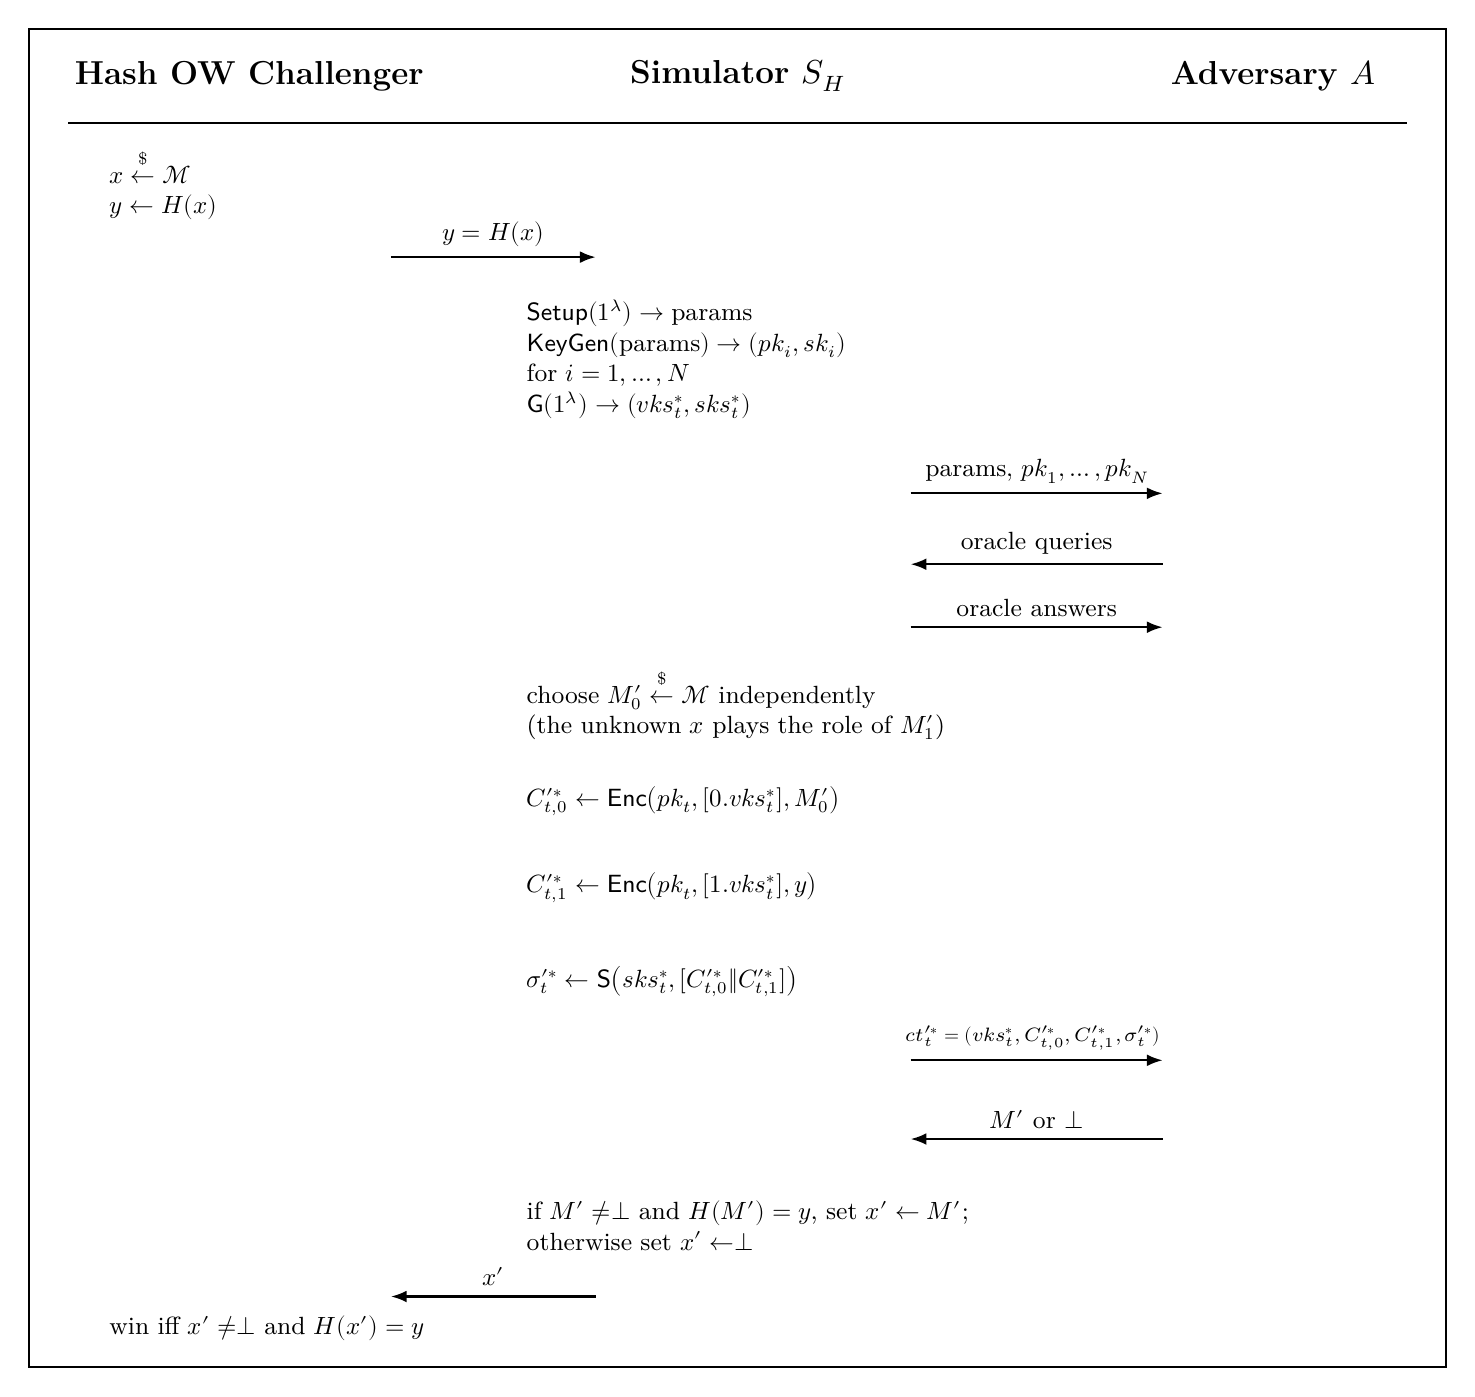
\begin{tikzpicture}[
    >=Latex,
    font=\small,
    header/.style={font=\bfseries\large},
    localhash/.style={align=left, text width=4.2cm},
    localsim/.style={align=left, text width=5.7cm},
    arr/.style={-{Latex[length=2mm]}, thick}
]

% =====================================================
% Fixed stakeholder columns
% =====================================================

\def\xHash{2.8}
\def\xSim{9.0}
\def\xAdv{15.8}

% Arrow zones between columns
\def\xHSL{4.6}
\def\xHSR{7.2}

\def\xSAL{11.2}
\def\xSAR{14.4}

% =====================================================
% Outer box
% =====================================================

\draw[thick] (0,0) rectangle (18,-17.0);
\draw[thick] (0.5,-1.2) -- (17.5,-1.2);

% =====================================================
% Headers
% =====================================================

\node[header] at (\xHash,-0.6)
{Hash OW Challenger};

\node[header] at (\xSim,-0.6)
{Simulator $S_H$};

\node[header] at (\xAdv,-0.6)
{Adversary $A$};

% =====================================================
% One-way hash challenge
% =====================================================

\node[localhash, anchor=west] at (0.9,-2.0)
{
$x \overset{\$}{\leftarrow} \mathcal{M}$\\
$y \gets H(x)$
};

\draw[arr]
    (\xHSL,-2.9)
    --
    node[above] {$y=H(x)$}
    (\xHSR,-2.9);

% =====================================================
% Simulator setup
% Same as a normal Game 1 challenger
% =====================================================

\node[localsim, anchor=west] at (6.2,-4.2)
{
$\mathsf{Setup}(1^\lambda)
 \rightarrow \mathrm{params}$\\
$\mathsf{KeyGen}(\mathrm{params})
 \rightarrow (pk_i,sk_i)$\\
for $i=1,\ldots,N$\\
$\mathsf{G}(1^\lambda)
 \rightarrow (vks_t^*,sks_t^*)$
};

\draw[arr]
    (\xSAL,-5.9)
    --
    node[above]
    {$\mathrm{params},\,pk_1,\ldots,pk_N$}
    (\xSAR,-5.9);

% =====================================================
% Oracle interactions
% =====================================================

\draw[arr]
    (\xSAR,-6.8)
    --
    node[above] {oracle queries}
    (\xSAL,-6.8);

\draw[arr]
    (\xSAL,-7.6)
    --
    node[above] {oracle answers}
    (\xSAR,-7.6);

% =====================================================
% Anomalous challenge construction
% =====================================================

\node[localsim, anchor=west] at (6.2,-8.6)
{
choose $M_0'
\overset{\$}{\leftarrow}\mathcal{M}$ independently\\
(the unknown $x$ plays the role of $M_1'$)
};

\node[localsim, anchor=west] at (6.2,-9.8)
{
$C_{t,0}^{\prime *}
 \gets
 \mathsf{Enc}\bigl(
    pk_t,
    [0.vks_t^*],
    M_0'
 \bigr)$
};

\node[localsim, anchor=west] at (6.2,-10.9)
{
$C_{t,1}^{\prime *}
 \gets
 \mathsf{Enc}\bigl(
    pk_t,
    [1.vks_t^*],
    y
 \bigr)$
};

\node[localsim, anchor=west] at (6.2,-12.1)
{
$\sigma_t^{\prime *}
 \gets
 \mathsf{S}\!\left(
    sks_t^*,
    [C_{t,0}^{\prime *}
     \Vert
     C_{t,1}^{\prime *}]
 \right)$
};

% =====================================================
% Challenge ciphertext
% =====================================================

\draw[arr]
    (\xSAL,-13.1)
    --
    node[
        midway,
        above,
        align=center,
        font=\scriptsize
    ]
    {
    $ct_t^{\prime *}
     =
     (vks_t^*,
      C_{t,0}^{\prime *},
      C_{t,1}^{\prime *},
      \sigma_t^{\prime *})$
    }
    (\xSAR,-13.1);

% =====================================================
% Adversary output
% =====================================================

\draw[arr]
    (\xSAR,-14.1)
    --
    node[above] {$M'$ or $\perp$}
    (\xSAL,-14.1);

% =====================================================
% Preimage verification
% =====================================================

\node[localsim, anchor=west] at (6.2,-15.2)
{
if $M'\neq\perp$ and $H(M')=y$, set
$x'\gets M'$;\\
otherwise set $x'\gets\perp$
};

% =====================================================
% Output to hash challenger
% =====================================================

\draw[arr]
    (\xHSR,-16.1)
    --
    node[above] {$x'$}
    (\xHSL,-16.1);

\node[localhash, anchor=west] at (0.9,-16.5)
{
win iff $x'\neq\perp$ and $H(x')=y$
};

\end{tikzpicture}

\caption{
Reduction from the pre-simulation to the one-wayness
of the hash function $H$.
The simulator $S_H$ embeds the challenge value
$y=H(x)$ into the second HIBE ciphertext component.
}
\label{fig:hash-ow-reduction}

\end{figure}

we have:

\[
Pr[A\rightarrow M_1' in PS] \le \epsilon_H
\]

% \begin{verbatim}
% Hash OW Challenger             Simulator S_H                 Adversary A
%         |                            |                            |
%         |---- y = H(x) ------------->|                            |
%         |                            |                            |
%         |                            |---- params, pks ---------->|
%         |                            |<--- oracle queries --------|
%         |                            |---- answers -------------->|
%         |                            |                            |
%         |                            | choose random M0'          |
%         |                            | C0' = Enc([0.vks*], M0')   |
%         |                            | C1' = Enc([1.vks*], y)     |
%         |                            | sigma'=Sign(C0'||C1')      |
%         |                            |---- ct' ------------------>|
%         |                            |                            |
%         |                            |<--- output M' -------------|
%         |<--- output M' as preimage -|                            |
% \end{verbatim}
\begin{figure}[ht]
\centering

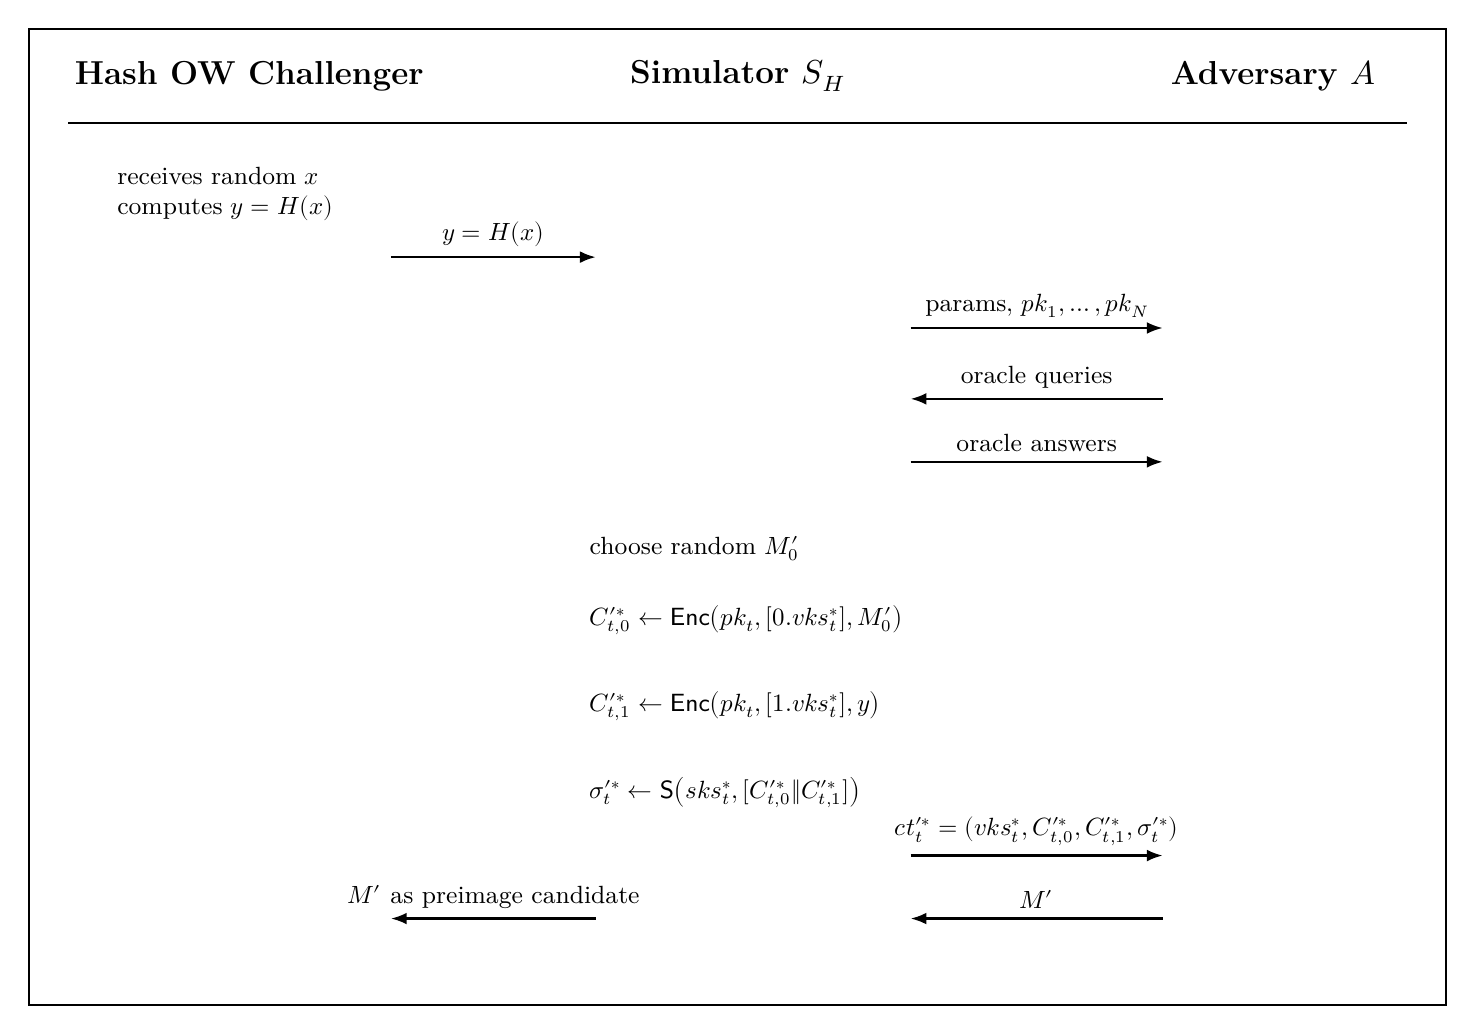
\begin{tikzpicture}[
    >=Latex,
    font=\small,
    header/.style={font=\bfseries\large},
    local/.style={align=left, text width=4.0cm},
    arr/.style={-{Latex[length=2mm]}, thick}
]

% =====================================================
% Fixed stakeholder columns
% =====================================================

\def\xHash{2.8}   % Hash challenger column center
\def\xSim{9.0}    % Simulator column center
\def\xAdv{15.8}   % Adversary column center

% Arrow zones between columns
\def\xHSL{4.6}    % between Hash challenger and Simulator
\def\xHSR{7.2}

\def\xSAL{11.2}   % between Simulator and Adversary
\def\xSAR{14.4}

% =====================================================
% Outer box
% =====================================================

\draw[thick] (0,0) rectangle (18,-12.4);
\draw[thick] (0.5,-1.2) -- (17.5,-1.2);

% =====================================================
% Headers
% =====================================================

\node[header] at (\xHash,-0.6) {Hash OW Challenger};
\node[header] at (\xSim,-0.6) {Simulator $S_H$};
\node[header] at (\xAdv,-0.6) {Adversary $A$};

% =====================================================
% Hash challenge setup
% =====================================================

\node[local, anchor=west] at (1.0,-2.1)
{
receives random $x$\\
computes $y = H(x)$
};

\draw[arr]
    (\xHSL,-2.9)
    --
    node[above] {$y=H(x)$}
    (\xHSR,-2.9);

% =====================================================
% Normal setup to A
% =====================================================

\draw[arr]
    (\xSAL,-3.8)
    --
    node[above] {$\mathrm{params},\,pk_1,\ldots,pk_N$}
    (\xSAR,-3.8);

\draw[arr]
    (\xSAR,-4.7)
    --
    node[above] {oracle queries}
    (\xSAL,-4.7);

\draw[arr]
    (\xSAL,-5.5)
    --
    node[above] {oracle answers}
    (\xSAR,-5.5);

% =====================================================
% Internal computation of simulator
% =====================================================

\node[local, anchor=west] at (7.0,-6.6)
{
choose random $M'_0$
};

\node[local, anchor=west] at (7.0,-7.5)
{
$C_{t,0}^{\prime *}
 \gets
 \mathsf{Enc}\bigl(pk_t,[0.vks_t^*],M'_0\bigr)$
};

\node[local, anchor=west] at (7.0,-8.6)
{
$C_{t,1}^{\prime *}
 \gets
 \mathsf{Enc}\bigl(pk_t,[1.vks_t^*],y\bigr)$
};

\node[local, anchor=west] at (7.0,-9.7)
{
$\sigma_t^{\prime *}
 \gets
 \mathsf{S}\!\left(
   sks_t^*,
   [C_{t,0}^{\prime *}\Vert C_{t,1}^{\prime *}]
 \right)$
};

% =====================================================
% Challenge ciphertext
% =====================================================

\draw[arr]
    (\xSAL,-10.5)
    --
    node[above]
    {$ct_t^{\prime *}
      =
      (vks_t^*,C_{t,0}^{\prime *},C_{t,1}^{\prime *},\sigma_t^{\prime *})$}
    (\xSAR,-10.5);

% =====================================================
% Adversary output and reduction output
% =====================================================

\draw[arr]
    (\xSAR,-11.3)
    --
    node[above] {$M'$}
    (\xSAL,-11.3);

\draw[arr]
    (\xHSR,-11.3)
    --
    node[above] {$M'$ as preimage candidate}
    (\xHSL,-11.3);

\end{tikzpicture}

\caption{
Reduction to the one-wayness of the hash function $H$.
The simulator $S_H$ embeds the hash challenge value $y=H(x)$
into the second component of the anomalous challenge ciphertext.
}
\label{fig:hash-ow-reduction}

\end{figure}
Security Game:

% \begin{verbatim}
% C_HIBE                         S_HIBE                              A
%    |                              |                                |
%    |                              | generate (vks_t*, sks_t*)      |
%    |                              | target ID = [0.vks_t*]         |
%    |<--- target ID [0.vks_t*] ----|                                |
%    |                              |                                |
%    |---- mpk -------------------->|                                |
%    |                              | set pk_t = mpk                 |
%    |                              | generate (pk_i,sk_i), i != t   |
%    |                              |---- params, all pk_i --------->|
%    |                              |                                |
%    |                              |<--- oracle queries ------------|
%    |                              |---- oracle answers ----------->|
%    |                              |                                |
%    |                              | choose random M0, M1           |
%    |<--- challenge M0, M1 --------|                                |
%    |---- C_{t,0,b}* ------------->|                                |
%    |                              | choose random beta             |
%    |                              | C_{t,1,beta}*=Enc([1.vks*],H(M_beta))
%    |                              | sigma*=Sign(C0*||C1*)          |
%    |                              |---- ct_t* -------------------->|
%    |                              |                                |
%    |                              |<--- A outputs M' or ⊥ ---------|
%    |                              | if M'=M_beta: output b'=beta   |
%    |                              | else: output random b'         |
%    |---- b' --------------------->|                                |
% \end{verbatim}


\begin{figure}[H]
\centering

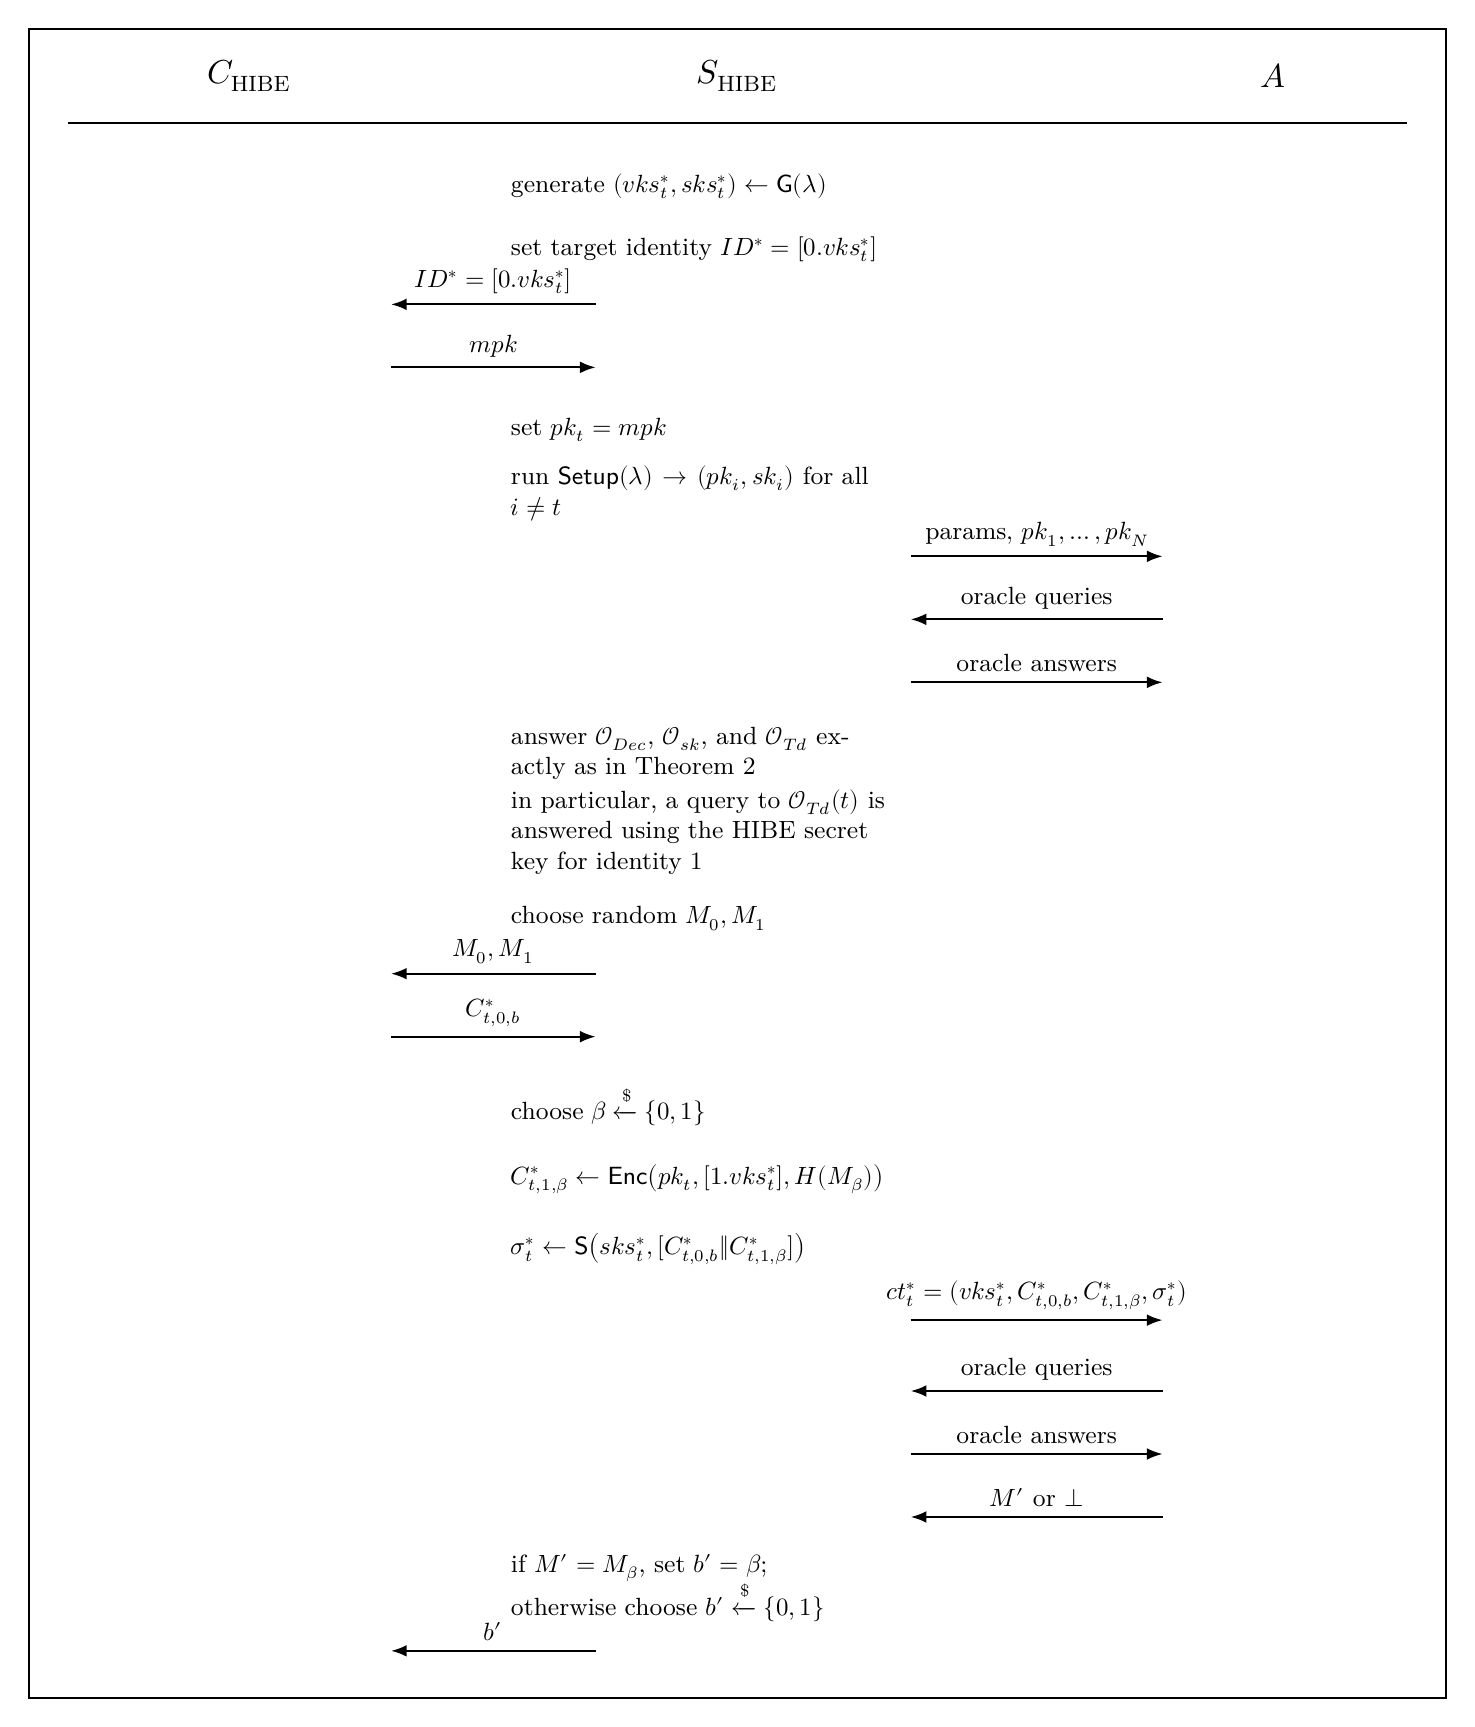
\begin{tikzpicture}[
    >=Latex,
    font=\small,
    header/.style={font=\bfseries\large},
    local/.style={align=left, text width=4.8cm},
    arr/.style={-{Latex[length=2mm]}, thick}
]

% =====================================================
% Fixed stakeholder columns
% =====================================================

\def\xChal{2.8}   % C_HIBE
\def\xSim{9.0}    % S_HIBE
\def\xAdv{15.8}   % A

% Arrow zones between columns
\def\xCSL{4.6}    % between challenger and simulator
\def\xCSR{7.2}

\def\xSAL{11.2}   % between simulator and adversary
\def\xSAR{14.4}

% =====================================================
% Outer box
% =====================================================

\draw[thick] (0,0) rectangle (18,-21.2);
\draw[thick] (0.5,-1.2) -- (17.5,-1.2);

% =====================================================
% Headers
% =====================================================

\node[header] at (\xChal,-0.6) {$C_{\mathrm{HIBE}}$};
\node[header] at (\xSim,-0.6) {$S_{\mathrm{HIBE}}$};
\node[header] at (\xAdv,-0.6) {$A$};

% =====================================================
% Initialization
% =====================================================

\node[local, anchor=west] at (6.0,-2.0)
{
generate $(vks_t^{*},sks_t^{*}) \gets \mathsf{G}(\lambda)$
};

\node[local, anchor=west] at (6.0,-2.8)
{
set target identity $ID^{*}=[0.vks_t^{*}]$
};

% S_HIBE -> C_HIBE : target identity
\draw[arr]
    (\xCSR,-3.5)
    --
    node[above] {$ID^{*}=[0.vks_t^{*}]$}
    (\xCSL,-3.5);

% C_HIBE -> S_HIBE : mpk
\draw[arr]
    (\xCSL,-4.3)
    --
    node[above] {$mpk$}
    (\xCSR,-4.3);

\node[local, anchor=west] at (6.0,-5.1)
{
set $pk_t = mpk$
};

\node[local, anchor=west] at (6.0,-5.9)
{
run $\mathsf{Setup}(\lambda)\to(pk_i,sk_i)$ for all $i\neq t$
};

% =====================================================
% Give public data to A
% =====================================================

\draw[arr]
    (\xSAL,-6.7)
    --
    node[above] {$\mathrm{params},\,pk_1,\ldots,pk_N$}
    (\xSAR,-6.7);

% =====================================================
% Oracle phase before challenge
% =====================================================

\draw[arr]
    (\xSAR,-7.5)
    --
    node[above] {oracle queries}
    (\xSAL,-7.5);

\draw[arr]
    (\xSAL,-8.3)
    --
    node[above] {oracle answers}
    (\xSAR,-8.3);

\node[local, anchor=west] at (6.0,-9.2)
{
answer $\mathcal{O}_{Dec}$, $\mathcal{O}_{sk}$, and $\mathcal{O}_{Td}$
exactly as in Theorem~2
};

\node[local, anchor=west] at (6.0,-10.2)
{
in particular, a query to $\mathcal{O}_{Td}(t)$ is answered
using the HIBE secret key for identity $1$
};

% =====================================================
% Challenge phase
% =====================================================

\node[local, anchor=west] at (6.0,-11.3)
{
choose random $M_0,M_1$
};

% S_HIBE -> C_HIBE : challenge messages
\draw[arr]
    (\xCSR,-12.0)
    --
    node[above] {$M_0,M_1$}
    (\xCSL,-12.0);

% C_HIBE -> S_HIBE : HIBE challenge ciphertext
\draw[arr]
    (\xCSL,-12.8)
    --
    node[above] {$C_{t,0,b}^{*}$}
    (\xCSR,-12.8);

\node[local, anchor=west] at (6.0,-13.7)
{
choose $\beta \xleftarrow{\$} \{0,1\}$
};

\node[local, anchor=west] at (6.0,-14.6)
{
$C_{t,1,\beta}^{*}
 \gets
 \mathsf{Enc}\bigl(pk_t,[1.vks_t^{*}],H(M_{\beta})\bigr)$
};

\node[local, anchor=west] at (6.0,-15.5)
{
$\sigma_t^{*}
 \gets
 \mathsf{S}\!\left(
   sks_t^{*},
   [C_{t,0,b}^{*}\Vert C_{t,1,\beta}^{*}]
 \right)$
};

% Send challenge ciphertext to A
\draw[arr]
    (\xSAL,-16.4)
    --
    node[above]
    {$ct_t^{*}=(vks_t^{*},C_{t,0,b}^{*},C_{t,1,\beta}^{*},\sigma_t^{*})$}
    (\xSAR,-16.4);

% =====================================================
% Oracle phase after challenge
% =====================================================

\draw[arr]
    (\xSAR,-17.3)
    --
    node[above] {oracle queries}
    (\xSAL,-17.3);

\draw[arr]
    (\xSAL,-18.1)
    --
    node[above] {oracle answers}
    (\xSAR,-18.1);

% =====================================================
% Final output
% =====================================================

\draw[arr]
    (\xSAR,-18.9)
    --
    node[above] {$M'$ or $\bot$}
    (\xSAL,-18.9);

\node[local, anchor=west] at (6.0,-19.8)
{
if $M'=M_{\beta}$, set $b'=\beta$;\\
otherwise choose $b' \xleftarrow{\$}\{0,1\}$
};

\draw[arr]
    (\xCSR,-20.6)
    --
    node[above] {$b'$}
    (\xCSL,-20.6);

\end{tikzpicture}

\caption{
Main simulation in the proof of Theorem~3:
the simulator $S_{\mathrm{HIBE}}$ uses adversary $A$
to attack the IND-sID-CPA security of the underlying HIBE scheme.
}
\label{fig:main-simulator-theorem3}
\end{figure}


\hypertarget{advantage-of-s_mathrmhibe}{%
\subsubsection{\texorpdfstring{Advantage of
\((S_{\mathrm{HIBE}})\)}{Advantage of (S\_\{\textbackslash mathrm\{HIBE\}\})}}\label{advantage-of-s_mathrmhibe}}

The advantage of \((S_{\mathrm{HIBE}})\) is:

\[
\begin{aligned}
\left|\Pr[b'=b]-\frac{1}{2}\right|
&=
\left|
\frac{1}{2}
\left(
\Pr[b'=b\mid b=\beta]
+
\Pr[b'=b\mid b\neq\beta]
\right)
-
\frac{1}{2}
\right| \\[2mm]
&=
\left|
\frac{1}{2}
\left(
\Pr[A\to M_b \vee (A\nrightarrow M_b \wedge b'=b)\mid b=\beta]
+
\Pr[b'=b\mid b\neq\beta]
\right)
-
\frac{1}{2}
\right| \\[2mm]
&=
\left|
\frac{1}{2}
\left(
\Pr[A\to M_b\mid b=\beta]
+
\Pr[A\nrightarrow M_b \wedge b'=b\mid b=\beta]
+
\Pr[b'=b\mid b\neq\beta]
\right)
-
\frac{1}{2}
\right| \\[2mm]
&=
\left|
\frac{1}{2}
\left(
\Pr[\mathcal{G}_1]
+
\frac{1}{2}\Pr[A\nrightarrow M_b\mid b=\beta]
+
\Pr[b'=b\mid b\neq\beta]
\right)
-
\frac{1}{2}
\right| \\[2mm]
&=
\left|
\frac{1}{2}
\left(
\Pr[\mathcal{G}_1]
+
\frac{1}{2}(1-\Pr[\mathcal{G}_1])
+
\Pr[b'=b\mid b\neq\beta]
\right)
-
\frac{1}{2}
\right| \\[2mm]
&=
\frac{1}{2}
\left|
\frac{1}{2}\Pr[\mathcal{G}_1]
+
\Pr[b'=b\mid b\neq\beta]
-
\frac{1}{2}
\right| \\[2mm]
&=
\frac{1}{2}
\left|
\frac{1}{2}\Pr[\mathcal{G}_1]
+
\Pr[A\nrightarrow M_\beta \wedge b'=b\mid b\neq\beta]
-
\frac{1}{2}
\right| \\[2mm]
&=
\frac{1}{2}
\left|
\frac{1}{2}\Pr[\mathcal{G}_1]
+
\frac{1}{2}\Pr[A\nrightarrow M_\beta\mid b\neq\beta]
-
\frac{1}{2}
\right| \\[2mm]
&=
\frac{1}{2}
\left|
\frac{1}{2}\Pr[\mathcal{G}_1]
+
\frac{1}{2}
\left(
1-\Pr[A\to M_\beta\mid b\neq\beta]
\right)
-
\frac{1}{2}
\right| \\[2mm]
&=
\frac{1}{4}
\left|
\Pr[\mathcal{G}_1]
-
\Pr[A\to M_\beta\mid b\neq\beta]
\right| \\[2mm]
&>
\frac{1}{4}
\left(
\Pr[\mathcal{G}_1]
-
\epsilon_H
\right).
\end{aligned}
\]

The last inequality follows from the pre-simulation result:

\[
\Pr[A\to M_\beta\mid b\neq\beta] < \epsilon_H.
\]

Therefore,

\[
Adv_{S_{\mathrm{HIBE}},HIBE}^{IND\text{-}sID\text{-}CPA}(\lambda)
>
\frac{1}{4}
\left(
\Pr[\mathcal{G}_1]
-
\epsilon_H
\right).
\]

Since

\[
\epsilon_1=\Pr[\mathcal{G}_1],
\]

we obtain:

\[
Adv_{S_{\mathrm{HIBE}},HIBE}^{IND\text{-}sID\text{-}CPA}(\lambda)
>
\frac{1}{4}
(\epsilon_1-\epsilon_H).
\]

By the IND-sID-CPA security of HIBE, this advantage must be smaller than
\((\epsilon_{\mathrm{HIBE}})\). Hence:

\[
\frac{1}{4}
(\epsilon_1-\epsilon_H)
<
\epsilon_{\mathrm{HIBE}}.
\]

Equivalently,

\[
\epsilon_1
<
4\epsilon_{\mathrm{HIBE}}
+
\epsilon_H.
\]

\end{document}
